\documentclass[a4paper,12pt]{article}
\usepackage[fontset=none]{ctex}
\usepackage{geometry}
\usepackage{graphicx}
\usepackage{amsmath}
\usepackage{enumitem}
\usepackage{setspace}
\usepackage{fontspec}
\usepackage{booktabs}
\usepackage{caption}
\usepackage{array}

% 字体设置（与 docx 模板一致）
\setCJKmainfont{Songti SC}          % 宋体 - 正文默认
\setCJKsansfont{Heiti SC}            % 黑体 - 一级标题
\setCJKmonofont[AutoFakeBold]{STFangsong}          % 仿宋 - 注意事项
\setmainfont{Times New Roman}        % 英文默认

% 页面设置
\geometry{left=2.5cm, right=2.5cm, top=2.5cm, bottom=2.5cm}

% 去掉页码
\pagestyle{empty}

\begin{document}

% ========== 封面 ==========
\begin{center}
    \vspace*{2cm}
    {\fontsize{36pt}{43pt}\selectfont \textbf{物理实验报告}}
    \vspace{3cm}
\end{center}

\begin{center}
    \fontsize{16pt}{24pt}\selectfont
    \textbf{实验名称：铁磁材料的磁滞回线和基本磁化曲线\quad} \\[0.5em]
    \textbf{实验桌号：\_\_\_\_\_\_\_\_\_\_\_\_\_\_\_\_\_\_\_\_\_\_\_\_\_} \\[0.5em]
    \textbf{指导教师：\_\_\_\_\_\_\_\_\_\_\_\_\_\_\_\_\_\_\_\_\_\_\_\_\_}
\end{center}

\vspace{2cm}

\begin{center}
    \fontsize{14pt}{28pt}\selectfont
    \textbf{周次：\_\_\_\_\_\_\_\_\_\_\_\_\_\_\_\_\_\_\_\_\_\_\_\_\_\_\_\_\_\_\_\_\_} \\
    \textbf{姓名：\_\_\_\_\_\_\_\_\_\_\_\_\_\_\_\_\_\_\_\_\_\_\_\_\_\_\_\_\_\_\_\_\_} \\
    \textbf{学号：\_\_\_\_\_\_\_\_\_\_\_\_\_\_\_\_\_\_\_\_\_\_\_\_\_\_\_\_\_\_\_\_\_} \\[0.5em]
    \textbf{实验日期: \_\_\_\_年\_\_\_\_月\_\_\_\_日\quad 星期\_\_\_上/下午}
\end{center}

\vspace{1.5cm}

\begin{center}
    \fontsize{14pt}{20pt}\selectfont
    浙江大学物理实验教学中心
\end{center}

\newpage

% ========== 一、预习报告 ==========
{\CJKfontspec{Heiti SC}\fontsize{16pt}{24pt}\selectfont \textbf{一、预习报告}}

\vspace{0.5cm}
{\fontsize{14pt}{20pt}\selectfont \textbf{1. 实验综述}}

\vspace{0.3cm}

{\fontsize{12pt}{18pt}\selectfont

铁磁材料（如Fe、Co、Ni及其合金）内部存在自发磁化的磁畴结构。在外磁场$H$作用下，磁畴旋转和畴壁迁移使材料被磁化，磁感应强度$B$随$H$增大而增大直至饱和。当$H$周期性变化时，$B$的变化滞后于$H$，形成磁滞回线，其包围面积反映磁滞损耗。磁滞回线的特征参数包括饱和磁感应强度$B_s$、剩余磁感应强度$B_r$和矫顽力$H_c$。

本实验采用\textbf{转换法}，利用示波器的X-Y模式显示B-H曲线。将铁磁样品置于交流励磁电路中，通过电阻$R_1$两端电压反映磁场强度$H$（X通道），通过RC积分电路的电容$C$两端电压反映磁感应强度$B$（Y通道）。逐步改变交流励磁电压，测量不同磁滞回线端点坐标，获得基本磁化曲线；在最大励磁电压下记录完整磁滞回线数据，并用Origin软件绘图和计算磁滞损耗。

}

\vspace{0.5cm}

{\fontsize{14pt}{20pt}\selectfont \textbf{2. 实验重点}}

\vspace{0.3cm}

{\fontsize{12pt}{18pt}\selectfont

掌握磁滞、磁滞回线和磁化曲线的基本概念，理解转换法的原理；学会利用示波器X-Y模式测绘B-H曲线，正确读取饱和磁感应强度$B_s$、剩磁$B_r$和矫顽力$H_c$等特征参数。

}

\vspace{0.5cm}

{\fontsize{14pt}{20pt}\selectfont \textbf{3. 实验难点}}

\vspace{0.3cm}

{\fontsize{12pt}{18pt}\selectfont

正确搭建交流励磁和RC积分电路，理解示波器电压信号到$H$和$B$的量纲转换关系；退磁操作的规范性（电压须单调降至0V）；利用Origin软件计算磁滞回线包围面积以求磁滞损耗。

}

\newpage

% ========== 二、原始数据 ==========
{\CJKfontspec{Heiti SC}\fontsize{16pt}{24pt}\selectfont \textbf{二、原始数据}}

\vspace{0.3cm}
{\fontsize{12pt}{18pt}\selectfont （将有学生和老师签名的"自备数据记录草稿纸"的扫描或手机拍摄图粘贴在下方）}

\vspace{0.5cm}

{\fontsize{12pt}{18pt}\selectfont

\textbf{实验参数：}$N_1 = N_2 = 150$T，$L = 6.0 \times 10^{-2}$\,m，$S = 8.0 \times 10^{-5}$\,m$^2$，$R_1 = 2.50\,\Omega$，$R_2 = 10\,$k$\Omega$，$C = 3.0\,\mu$F，$f = 130$\,Hz。

\textbf{换算公式：}
\begin{equation}
H = \frac{N_1 U_1}{L R_1} \quad(\text{A/m}), \qquad
B = \frac{R_2 C U_2}{N_2 S} \quad(\text{T})
\end{equation}

代入参数后简化为：$H\,(\text{A/m}) = U_1\,(\text{mV})$，$B\,(\text{mT}) = 2.5 \times U_2\,(\text{mV})$。

}

\vspace{0.5cm}

{\fontsize{12pt}{18pt}\selectfont \textbf{表1：初始磁化曲线数据}}

\vspace{0.3cm}

\begin{table}[h]
\centering
\fontsize{10pt}{14pt}\selectfont
\begin{tabular}{c c c c c c}
\toprule
$U$/V & $H$/（A/m） & $B$/mT & $\mu = B/H$/（mT$\cdot$m/A） & $U_1$/mV & $U_2$/mV \\
\midrule
0.5  & 55.02  & 107.80 & 1.9593 & 55.02  & 43.12 \\
1.0  & 97.54  & 216.77 & 2.2224 & 97.54  & 86.71 \\
1.2  & 117.80 & 257.75 & 2.1880 & 117.80 & 103.10 \\
1.5  & 150.60 & 324.00 & 2.1514 & 150.60 & 129.60 \\
1.8  & 186.60 & 388.50 & 2.0820 & 186.60 & 155.40 \\
2.0  & 216.90 & 445.25 & 2.0528 & 216.90 & 178.10 \\
2.2  & 248.20 & 488.25 & 1.9672 & 248.20 & 195.30 \\
2.5  & 301.30 & 550.75 & 1.8279 & 301.30 & 220.30 \\
2.8  & 370.00 & 617.00 & 1.6676 & 370.00 & 246.80 \\
3.0  & 423.20 & 656.25 & 1.5507 & 423.20 & 262.50 \\
\bottomrule
\end{tabular}
\end{table}

\vspace{0.5cm}

{\fontsize{12pt}{18pt}\selectfont \textbf{表2：动态磁滞回线数据（励磁电压3.0V）}}

\vspace{0.3cm}

\begin{table}[h]
\centering
\fontsize{10pt}{14pt}\selectfont
\begin{tabular}{c c c c c}
\toprule
NO & $H$/（A/m） & $B$/mT & $U_1$/mV & $U_2$/mV \\
\midrule
1  & 0.00     & 234.38  & 0      & 93.75  \\
2  & 28.12    & 277.25  & 28.12  & 110.90 \\
3  & 50.00    & 320.25  & 50.00  & 128.10 \\
4  & 78.12    & 363.25  & 78.12  & 145.30 \\
5  & 106.20   & 406.25  & 106.20 & 162.50 \\
6  & 140.60   & 441.25  & 140.60 & 176.50 \\
7  & 190.60   & 496.00  & 190.60 & 198.40 \\
8  & 240.60   & 535.00  & 240.60 & 214.00 \\
9  & 306.20   & 578.00  & 306.20 & 231.20 \\
10 & 353.10   & 609.25  & 353.10 & 243.70 \\
11 & 390.60   & 632.75  & 390.60 & 253.10 \\
12 & 418.70   & 648.25  & 418.70 & 259.30 \\
13 & 378.10   & 597.50  & 378.10 & 239.00 \\
14 & 337.50   & 570.25  & 337.50 & 228.10 \\
15 & 306.20   & 519.50  & 306.20 & 207.80 \\
16 & 271.80   & 488.25  & 271.80 & 195.30 \\
17 & 243.70   & 453.00  & 243.70 & 181.20 \\
18 & 218.70   & 402.25  & 218.70 & 160.90 \\
19 & 190.60   & 347.50  & 190.60 & 139.00 \\
20 & 165.60   & 281.25  & 165.60 & 112.50 \\
21 & 140.60   & 230.45  & 140.60 & 92.18  \\
22 & 115.60   & 148.42  & 115.60 & 59.37  \\
23 & 103.10   & 89.83   & 103.10 & 35.93  \\
24 & 90.62    & 23.44   & 90.62  & 9.374  \\
25 & $-$25.00 & 144.53  & $-$25.00 & 57.81 \\
26 & $-$43.75 & 101.55  & $-$43.75 & 40.62 \\
27 & $-$56.25 & 70.30   & $-$56.25 & 28.12 \\
28 & $-$68.75 & 35.15   & $-$68.75 & 14.06 \\
\bottomrule
\end{tabular}
\end{table}

\vspace{0.3cm}

{\fontsize{12pt}{18pt}\selectfont

\textbf{磁滞回线特征参数：}

矫顽力 $H_c = 70.09$\,A/m，剩余磁感应强度 $B_r = 234.38$\,mT，

饱和磁感应强度 $B_m = 648.25$\,mT，磁滞损耗 $[BH] = 105.72$\,J/m$^3$。

}

\newpage

% ========== 三、结果与分析 ==========
{\CJKfontspec{Heiti SC}\fontsize{16pt}{24pt}\selectfont \textbf{三、结果与分析}}

\vspace{0.5cm}
{\fontsize{14pt}{20pt}\selectfont \textbf{1. 数据处理与结果}}

\vspace{0.3cm}

{\fontsize{12pt}{18pt}\selectfont

\textbf{（1）基本磁化曲线：}

根据表1数据，以$H$为横轴，分别以$B$和$\mu = B/H$为纵轴，绘制双Y轴磁化曲线图（图1）。

由图可见，$B$随$H$增加呈现先快后慢的饱和趋势，在$H \approx 420$\,A/m时$B$趋于饱和（$B_m \approx 656$\,mT）。$\mu = B/H$先升后降，在$H \approx 100$\,A/m附近取得最大值（$\mu_{\max} \approx 2.22$\,mT$\cdot$m/A），随后由于铁磁材料逐渐接近磁饱和而单调下降。

\begin{figure}[h]
\centering
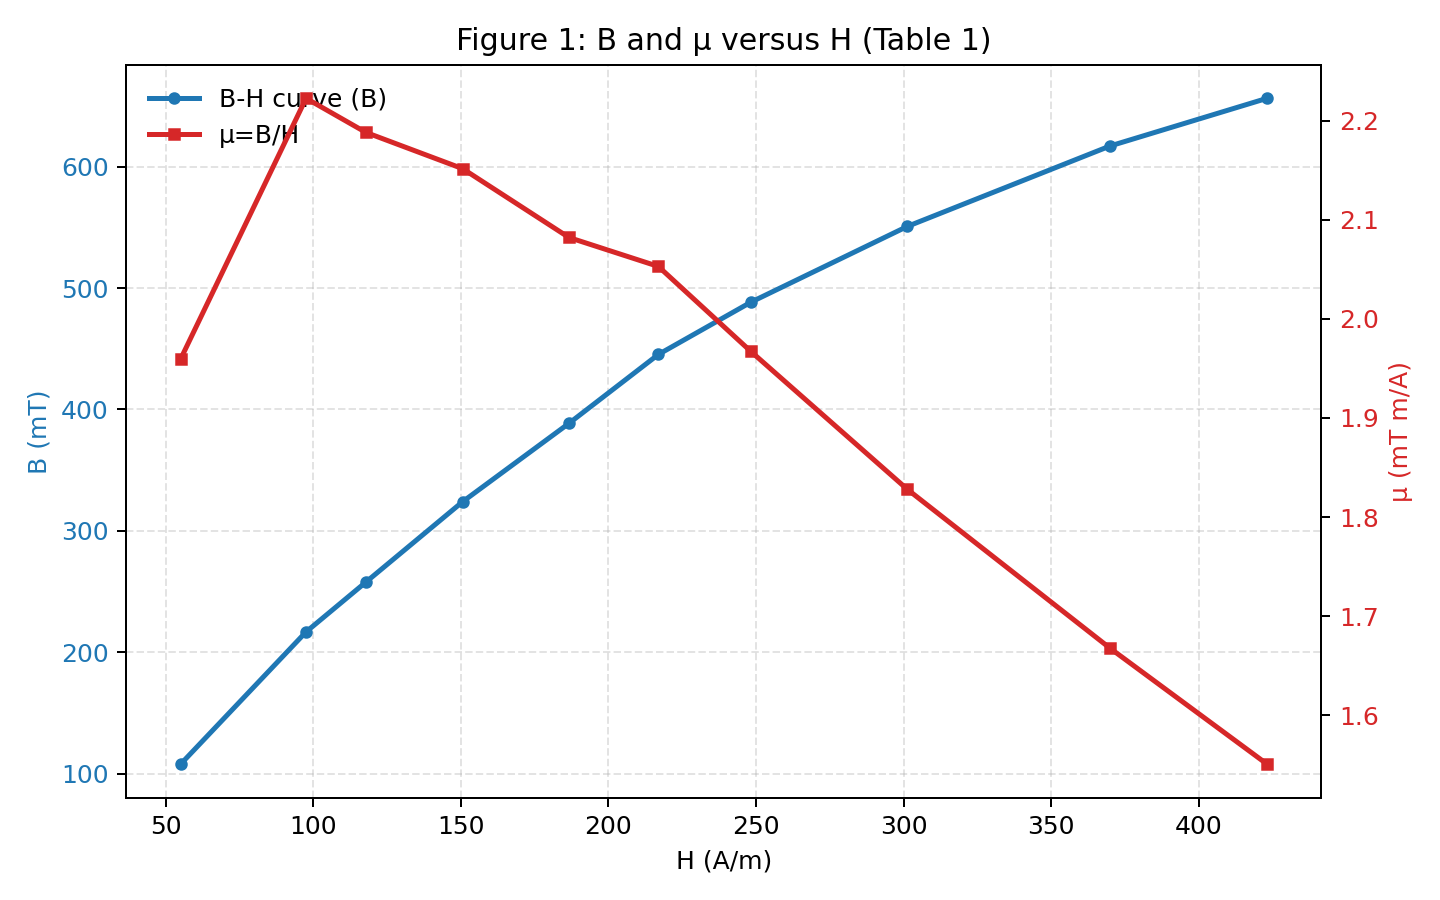
\includegraphics[width=0.85\textwidth]{../figure1_B_mu_vs_H.png}
\caption{$B$和$\mu$随$H$变化的双Y轴磁化曲线图}
\end{figure}

\textbf{（2）动态磁滞回线：}

根据表2数据，绘制磁滞回线图（图2）。由于磁滞回线关于原点中心对称，实测一半分支后通过对称映射补全另一半，得到完整闭合的磁滞回线。

由图可见磁滞回线呈典型的"S"形闭合曲线，$B$的变化明显滞后于$H$。从回线上读取特征参数：

\begin{itemize}[nosep]
    \item 饱和磁感应强度 $B_m = 648.25$\,mT（磁滞回线顶端）
    \item 剩余磁感应强度 $B_r = 234.38$\,mT（$H = 0$时的$B$值）
    \item 矫顽力 $H_c = 70.09$\,A/m（$B = 0$时的$H$值）
\end{itemize}

该样品的矫顽力$H_c$较小（$\sim 70$\,A/m），属于典型的\textbf{软磁材料}，适用于变压器、电动机铁芯等需反复磁化的场合。

\begin{figure}[h]
\centering
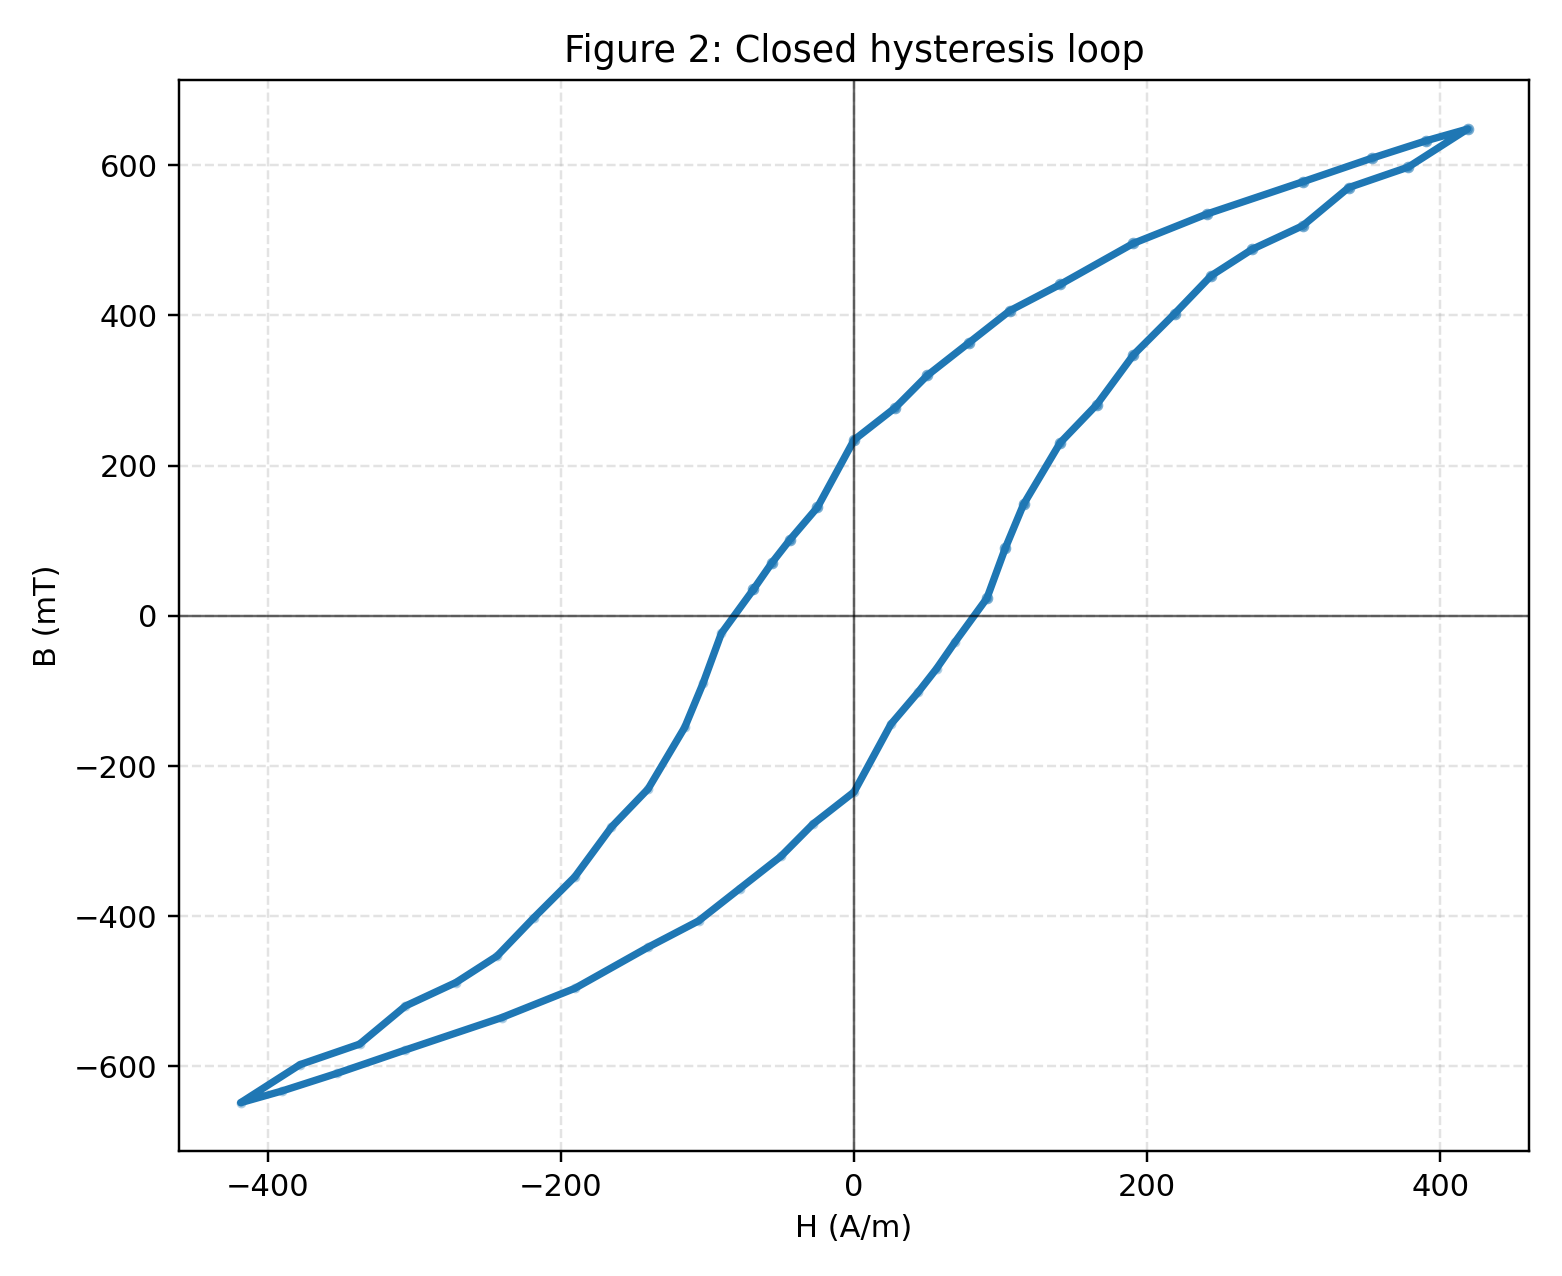
\includegraphics[width=0.75\textwidth]{../figure2_hysteresis_loop.png}
\caption{铁磁材料的动态磁滞回线图}
\end{figure}

\textbf{（3）磁滞损耗计算：}

磁滞损耗$[BH]$等于磁滞回线所包围面积。利用Shoelace公式（多边形面积法）对回线数据点计算闭合面积，由单侧分支面积乘以2得到完整回线面积：
\begin{equation}
[BH] = 2 \times \frac{1}{2}\left|\sum_{i=1}^{n}\left(H_i B_{i+1} - H_{i+1} B_i\right)\right| = 105.72 \quad \text{J/m}^3
\end{equation}

其中$B$在计算时需换算为T（$1\,\text{mT} = 10^{-3}\,\text{T}$），使结果单位为J/m$^3$。

}

\vspace{0.5cm}
{\fontsize{14pt}{20pt}\selectfont \textbf{2. 误差分析}}

\vspace{0.3cm}

{\fontsize{12pt}{18pt}\selectfont

\textbf{（1）系统误差：}

\begin{itemize}[nosep]
    \item 示波器读数精度有限，光标定位存在$\pm 1$\,mV级的读数误差，对应$H$约$\pm 1$\,A/m，$B$约$\pm 2.5$\,mT。
    \item 电阻$R_1$、$R_2$和电容$C$的标称值与实际值之间可能存在偏差，直接影响$H$和$B$的换算精度。
    \item 交流频率130\,Hz下的动态磁滞回线和准静态磁滞回线存在差异，频率效应会导致回线面积偏大。
\end{itemize}

\textbf{（2）随机误差：}

\begin{itemize}[nosep]
    \item 示波器光标读取过程中的人为定位误差。
    \item 交流励磁电压的波动导致$H$和$B$值在测量过程中存在微小变化。
\end{itemize}

\textbf{（3）相对误差估算：}

以$B_r$为例，示波器光标读数误差约为$\pm 1$\,mV（对应$U_2$），则$B_r$的相对误差为：
\begin{equation}
\frac{\Delta B_r}{B_r} = \frac{\Delta U_2}{U_2} = \frac{1}{93.75} \approx 1.1\%
\end{equation}

以$H_c$为例，若$U_1$读数误差约$\pm 1$\,mV，则相对误差为：
\begin{equation}
\frac{\Delta H_c}{H_c} = \frac{\Delta U_1}{U_1} \approx \frac{1}{70.09} \approx 1.4\%
\end{equation}

总体而言，本实验的系统误差和随机误差均较小，主要特征参数的相对误差在1\%--2\%量级。

}

\vspace{0.5cm}
{\fontsize{14pt}{20pt}\selectfont \textbf{3. 实验探讨}}

\vspace{0.3cm}

{\fontsize{12pt}{18pt}\selectfont

本实验通过转换法，利用示波器X-Y模式成功测绘了铁磁材料的基本磁化曲线和动态磁滞回线。实验结果表明该样品为软磁材料，具有较小的矫顽力和较窄的磁滞回线。磁化曲线中$\mu$先升后降的趋势与磁畴理论一致，验证了铁磁材料磁化过程中畴壁迁移到磁畴旋转的转变机制。

}

\newpage

% ========== 四、思考题 ==========
{\CJKfontspec{Heiti SC}\fontsize{16pt}{24pt}\selectfont \textbf{四、思考题}}

\vspace{0.5cm}

{\fontsize{12pt}{18pt}\selectfont

\textbf{1. $[BH]$（磁能积）的单位是否与能量有关？请给出量纲的推导过程。}

磁能积$[BH]$的单位为磁滞回线所围面积的单位，即$B$的单位乘以$H$的单位。在SI中，$[B] = \text{T} = \text{kg}\cdot\text{s}^{-2}\cdot\text{A}^{-1}$，$[H] = \text{A/m}$，因此：
\begin{equation}
[BH] = \text{T} \cdot \text{A/m} = \frac{\text{kg}}{\text{s}^2 \cdot \text{A}} \cdot \frac{\text{A}}{\text{m}} = \frac{\text{kg}}{\text{m} \cdot \text{s}^2} = \frac{\text{J}}{\text{m}^3}
\end{equation}
$[BH]$的量纲为能量/体积（J/m$^3$），即\textbf{能量密度}。它表征铁磁材料在一个磁化循环中单位体积的磁滞损耗能量，确实与能量直接相关。

\vspace{0.5cm}

\textbf{2. 查阅有关资料，简要回答积分电路的原理与有关应用。}

积分电路（RC积分电路）由电阻$R$和电容$C$串联组成，输出取自电容两端。当满足$RC \gg T$（$T$为信号周期）即$R \gg \dfrac{1}{\omega C}$时，电流近似为$i \approx u_{\text{in}}/R$，电容电压为：
\begin{equation}
u_{\text{out}} = \frac{1}{C}\int i\,dt \approx \frac{1}{RC}\int u_{\text{in}}\,dt
\end{equation}
输出信号正比于输入信号的时间积分。应用包括：（1）本实验中将感应电动势（$dB/dt$的信号）积分还原为$B$信号；（2）将方波转换为三角波（波形变换）；（3）模拟计算机中实现积分运算；（4）电子滤波器中用作低通滤波器，抑制高频噪声。

\vspace{0.5cm}

\textbf{3. 磁性材料内部的涡流损耗的能量是否可以被利用起来？请列出应用实例。}

可以。涡流损耗将电磁能转化为热能，虽然在变压器等设备中是有害损耗，但这一效应可以被有效利用：
\begin{itemize}[nosep]
    \item \textbf{电磁炉}：利用高频交变磁场在金属锅底感应涡流，涡流损耗产生的热量直接加热食物，热效率高。
    \item \textbf{工业感应加热}：金属冶炼、热处理和焊接中，利用涡流效应对金属工件进行快速均匀加热。
    \item \textbf{电磁制动}：涡流制动器利用导体在磁场中运动产生的涡流阻力实现无接触制动，应用于高速列车和卡车的辅助制动系统。
    \item \textbf{金属探测器}：通过检测涡流效应引起的磁场变化来探测金属物体的存在。
\end{itemize}

}

\vfill

% ========== 注意事项 ==========
\noindent\rule{\textwidth}{0.4pt}

{\CJKfontspec[AutoFakeBold]{STFangsong}\fontsize{12pt}{18pt}\selectfont
\textbf{注意事项：}
\begin{enumerate}[label=\arabic*., leftmargin=2em, nosep]
    \item 用PDF格式上传"实验报告"，文件名：学生姓名+学号+实验名称+周次。
    \item "实验报告"必须递交在"学在浙大"的本课程的对应实验项目的"作业"模块内。
    \item "实验报告"成绩必须在"浙江大学物理实验教学中心网站"-"选课系统"内查询。
    \item 教学评价必须在"浙江大学物理实验教学中心网站"-"选课系统"内进行，学生必须进行教学评价，才能看到实验报告成绩，教学评价必须在本次实验结束后3天内进行。
\end{enumerate}
}

\vspace{0.5cm}
\begin{center}
    {\CJKfontspec[AutoFakeBold]{STFangsong}\fontsize{12pt}{18pt}\selectfont \textbf{浙江大学物理实验教学中心制}}
\end{center}

\end{document}
